\documentclass[11pt, table]{beamer}
%\usepackage[table,x11names]{xcolor}
\usepackage[utf8]{inputenc}
\usepackage[T1]{fontenc}
\usepackage{multirow}
\usepackage{calc}
\usepackage{array}
\usepackage{graphicx}
\usepackage{multirow}

\newcommand{\p}{\pause}


\usetheme{default}

\newcommand\MyBox[2]{
	\fbox{\lower0.75cm
		\vbox to 1.7cm{\vfil
			\hbox to 1.7cm{\hfil\parbox{1.4cm}{#1\\#2}\hfil}
			\vfil}%
	}%
}

\begin{document}
	%\author{}
	\title{Introduction to Linear Regression}
	%\subtitle{}
	%\logo{}
	%\institute{}
	%\date{}
	%\subject{}
	%\setbeamercovered{transparent}
	%\setbeamertemplate{navigation symbols}{}
	\begin{frame}[plain]
	\maketitle
\end{frame}

\begin{frame}
\frametitle{Least-Squares Regression}
Let's say we're interested in houses near Belmont. We gather a sample of 20 homes in the area and look at sales prices for those homes.
\vspace{0.1in}

In our sample, we find that the average sales price was \$482,000.
\vspace{0.1in}

If we are trying to predict the price of another house in this area, what would our best guess be?\vspace{0.1in}\p

In the absence of other information, we could go with the average price from our sample, \$482,000, but could we do better if we had more information?
\end{frame}

\begin{frame}
\frametitle{Least-Squares Regression}
What if we also looked at the square footage of the homes in our sample. Here's a scatterplot of our sample:

\begin{center}
	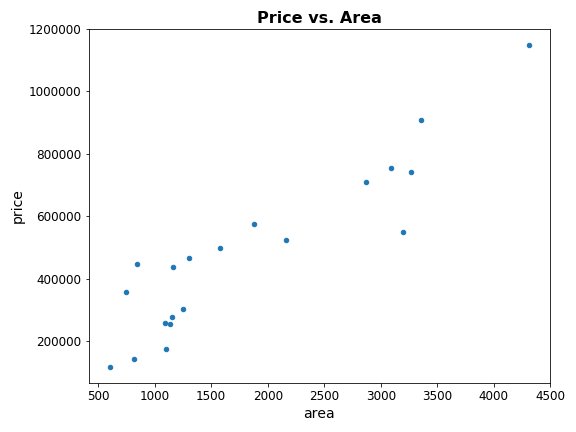
\includegraphics[width=2.5in]{images/Appraisal_Values/scatter.png}
\end{center}

If we know that a house we're interested in is 3200 sqft, could we now make a better guess versus just guessing the average price for the area?

\end{frame}


\begin{frame}
\frametitle{Least-Squares Regression}
The big idea of least-squares regression is to find a line which describes the relationship between two variables.
\vspace{0.1in}

Such a line will rarely completely describe the relationship since there will be some uncertainty due either to randomness of due to variables we did not measure.
\vspace{0.1in}

For example, the price of a home is never completely determined by the square footage, but we can probably make a decent guess about the price by knowing how large the house is.
\end{frame}

\begin{frame}
\frametitle{Least-Squares Regression}
There are many possible lines that we could use to try and describe the relationship between square footage and price.

\begin{center}
	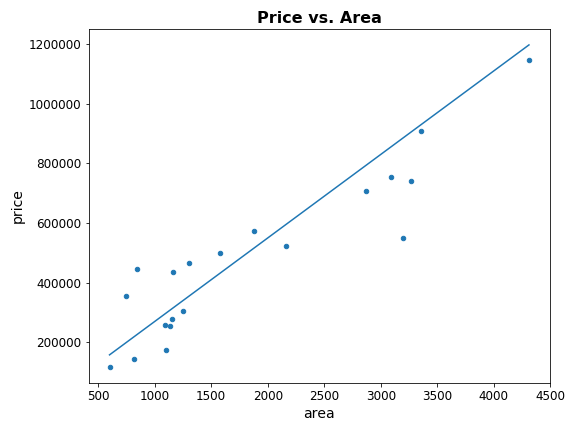
\includegraphics[width=2.5in]{images/Appraisal_Values/ols_01.png}
\end{center}

\end{frame}

\begin{frame}
\frametitle{Least-Squares Regression}
There are many possible lines that we could use to try and describe the relationship between square footage and price.

\begin{center}
	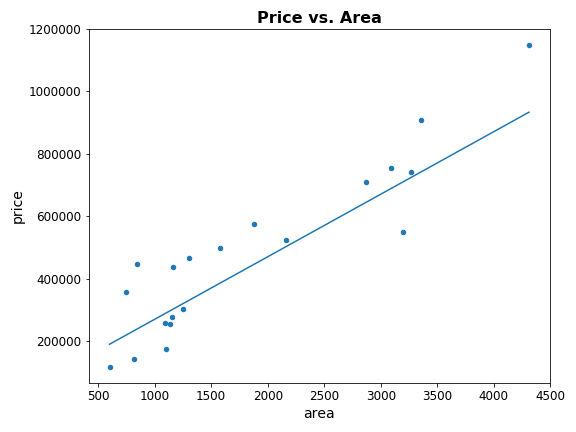
\includegraphics[width=2.5in]{images/Appraisal_Values/ols_02.png}
\end{center}

\end{frame}

\begin{frame}
\frametitle{Least-Squares Regression}
There are many possible lines that we could use to try and describe the relationship between square footage and price.

\begin{center}
	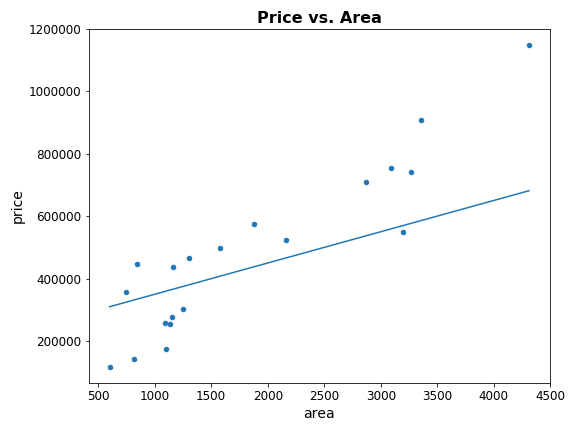
\includegraphics[width=2.5in]{images/Appraisal_Values/ols_03.png}
\end{center}
\end{frame}

\begin{frame}
\frametitle{Least-Squares Regression}
How do we choose the line to use out of all of the options?
\vspace{0.1in}

We'll choose by looking at the \textbf{residuals} - the vertical distance from the line to each point. In this case, the residuals represent the difference between the true price and what we would guess for the price is we used the line to predict price based on square footage.
\vspace{0.1in}

Because it makes the math work out nicer, we'll really be looking at the squared residuals, but we can get a pretty good idea by looking at the regular residuals.
\end{frame}

\begin{frame}
\frametitle{Least-Squares Regression}
There are many possible lines that we could use to try and describe the relationship between square footage and price.

\begin{center}
	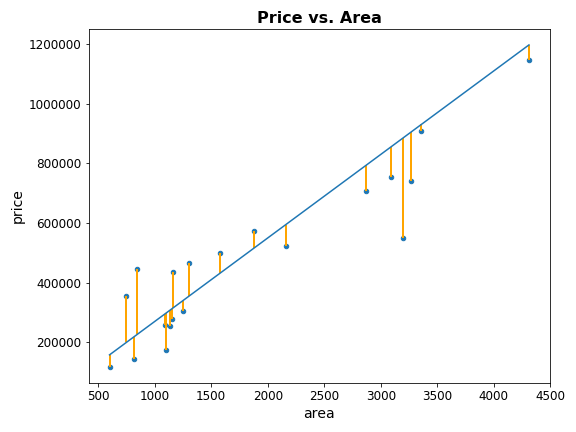
\includegraphics[width=2.5in]{images/Appraisal_Values/resid_01.png}
\end{center}
\end{frame}


\begin{frame}
\frametitle{Least-Squares Regression}
There are many possible lines that we could use to try and describe the relationship between square footage and price.

\begin{center}
	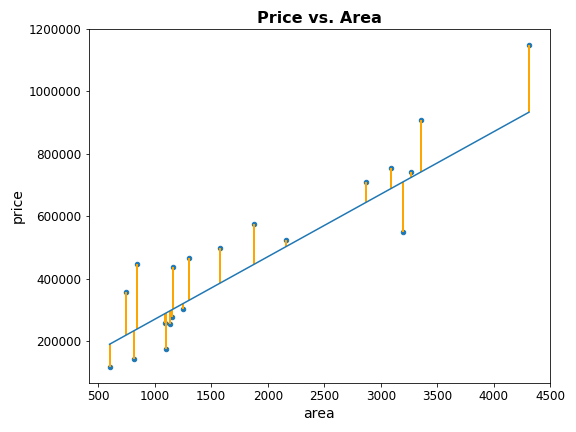
\includegraphics[width=2.5in]{images/Appraisal_Values/resid_02.png}
\end{center}
\end{frame}


\begin{frame}
\frametitle{Least-Squares Regression}
There are many possible lines that we could use to try and describe the relationship between square footage and price.

\begin{center}
	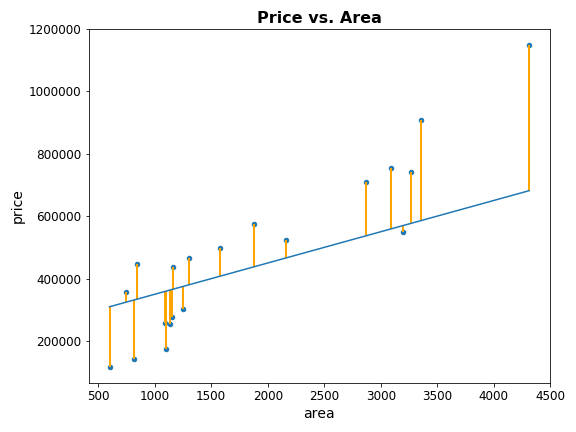
\includegraphics[width=2.5in]{images/Appraisal_Values/resid_03.png}
\end{center}
\end{frame}

\begin{frame}
\frametitle{Least-Squares Regression}
It turns out that the line with the smallest squared residuals is this one, with equation
$$\text{price} = 223.7\cdot(\text{sqft}) + 69522.4$$

\begin{center}
	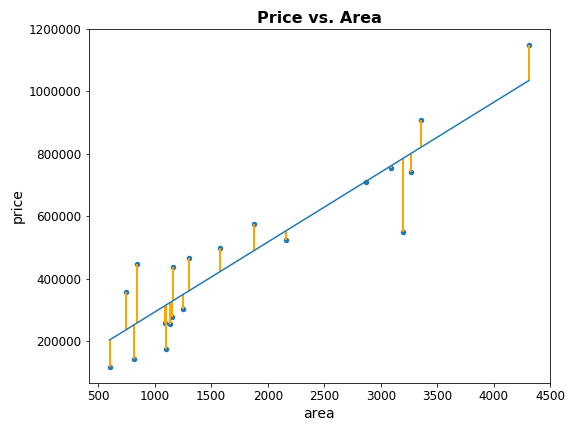
\includegraphics[width=2.5in]{images/Appraisal_Values/resid_04.png}
\end{center}
\end{frame}

\begin{frame}
\frametitle{Least-Squares Regression}
\textbf{Least-Squares Regression Line:}
$$\text{price} = 223.7\cdot(\text{sqft}) + 69522.4$$

This equation tells us that for every additional one square foot of area, the price tends to increase by about \$223.7. \p
\vspace{0.1in}

This mean that increasing the square footage of a house by 50 square feet will tend to increase the price by about\p
 $$50\cdot\$223.7\p = \$11,185$$
\end{frame}

\begin{frame}
\frametitle{Least-Squares Regression}
\textbf{Least-Squares Regression Line:}
$$\text{price} = 223.7\cdot(\text{sqft}) + 69522.4$$
Also, for a house that is 3200 sqft, we can expect the price to be around\p
$$ \$223.7\cdot 3200 + \$69522.4 \p = \$785,362.4$$\p

\begin{center}
	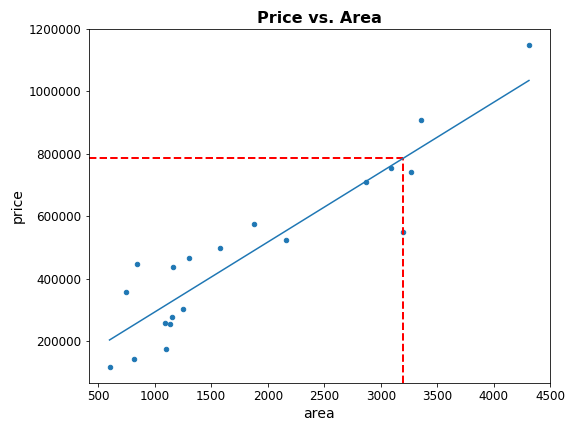
\includegraphics[width=2.5in]{images/Appraisal_Values/pred_01.png}
\end{center}

\end{frame}

\begin{frame}
\frametitle{Least-Squares Regression}
We can quantify how well our line fits the data by using the coefficient of determination, or $R^2$.
\vspace{0.1in}

We can understand $R^2$ by comparing the resiudals for our fitted line versus the residuals if we only used the average price to make our predictions.
\end{frame}

\begin{frame}
\frametitle{Least-Squares Regression}

\begin{center}
	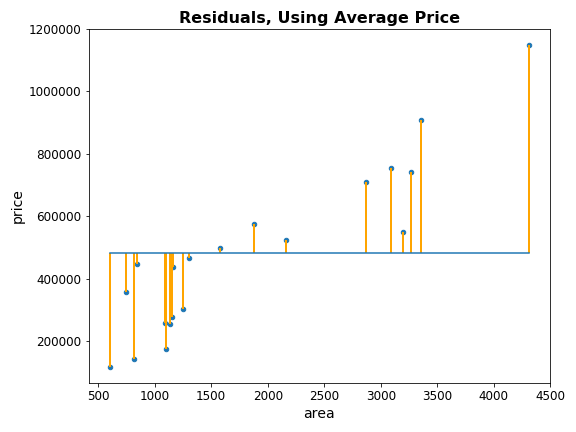
\includegraphics[width=3in]{images/Appraisal_Values/r2_01.png}
\end{center}

\end{frame}

\begin{frame}
\frametitle{Least-Squares Regression}

\begin{center}
	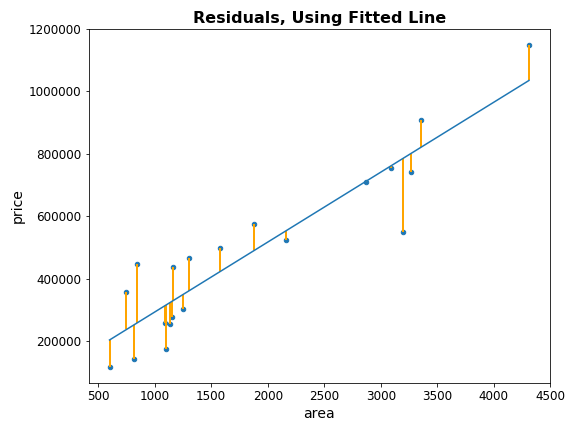
\includegraphics[width=3in]{images/Appraisal_Values/r2_02.png}
\end{center}

\end{frame}

\begin{frame}
\frametitle{Least-Squares Regression}
The coefficient of determination, $R^2$ roughly measures the proportion by which we reduce the residuals by using our the fitted line instead of just using the average price to predict.\p
\vspace{0.1in}

The coefficient of determination will take values between 0 and 1, with 1 representing a perfect fit.\p
\vspace{0.1in}

In this case, the residuals were reduced by a significant amount. Consequently, the $R^2$ value is equal to 0.842.
\end{frame}
\end{document}
